\documentclass[10pt,twocolumn,letterpaper]{article}

\usepackage{cvpr}
\usepackage{times}
\usepackage{epsfig}
\usepackage{graphicx}
\usepackage{amsmath}
\usepackage{amssymb}

% Include other packages here, before hyperref.

% If you comment hyperref and then uncomment it, you should delete
% egpaper.aux before re-running latex.  (Or just hit 'q' on the first latex
% run, let it finish, and you should be clear).
\usepackage[breaklinks=true,bookmarks=false]{hyperref}

\cvprfinalcopy % *** Uncomment this line for the final submission

\def\cvprPaperID{****} % *** Enter the CVPR Paper ID here
\def\httilde{\mbox{\tt\raisebox{-.5ex}{\symbol{126}}}}

% Pages are numbered in submission mode, and unnumbered in camera-ready
%\ifcvprfinal\pagestyle{empty}\fi
\setcounter{page}{4321}
\begin{document}

%%%%%%%%% TITLE
\title{Cost-Sensitive Loss Function Design for Credit Card Fraud Detection}

\author{Kevin Zong\\
{\tt\small kzong@umd.edu}
% For a paper whose authors are all at the same institution,
% omit the following lines up until the closing ``}''.
% Additional authors and addresses can be added with ``\and'',
% just like the second author.
% To save space, use either the email address or home page, not both
\and
Michael Obajemu\\
{\tt\small mobajemu@umd.edu}
\and
Emerald San\\
{\tt\small esan1@umd.edu}
}

\maketitle
%\thispagestyle{empty}

\section{Abstract}
Credit card fraud is characterized by extreme class imbalance (0.172\% fraud rate) and asymmetric misclassification costs,
 where missing a \$10,000 fraudulent transaction is far more costly than falsely flagging a \$10 legitimate one.
 Standard neural network loss functions treat all classification errors equally, ignoring the varying impact across transactions.
 We propose Amount-Weighted Cost-Sensitive Focal Loss (AWCS-FL), which extends focal loss by incorporating three components: 
 transaction amount weighting to prioritize expensive fraud, asymmetric business costs reflecting real operational expenses, 
 and temporal decay to adapt to evolving patterns. 

 We evaluate AWCS-FL on the Kaggle Credit Card Fraud Detection dataset against three baselines: binary cross-entropy, weighted BCE,
 and focal loss. Our method reduces financial losses by 34\% while achieving  77\% fraud prevention, though with lower precision than
  focal loss. Ablation studies confirm that cost sensitivity and amount weighting drive most of the improvement, with temporal weighting contributing minimally.
  Our results demonstrate that directly optimizing for business objectives substantially reduces financial losses but trades off against statistical metrics like F1 score.

%------------------------------------------------------------------------
\section{Introduction}

The widespread adoption of credit cards has led to a significant increase in fraud, costing financial institutions billions of dollars annually [1]. Effective fraud detection systems are essential for minimizing these losses while maintaining customer trust. This paper addresses the problem of credit card fraud detection using machine learning techniques.
Fraud detection is fundamentally a classification problem, where the objective is to distinguish fraudulent transactions from legitimate ones. However, this task presents several unique challenges. First, datasets are extremely imbalanced, with fraudulent transactions typically representing less than 1\% of all transactions. Second, the cost of misclassificationis 
highly asymmetric. Missing a fraudulent transaction results in significant financial losses, while incorrectly flagging a legitimate transaction primarily causes customer inconvenience and operational overhead. Third, not all errors are equal. Missing a \$10,000 fraudulent transaction has far greater business impact than missing a \$10 transaction, yet standard machine learning approaches treat these errors identically.
We propose a novel loss function called Amount-Weighted Cost-Sensitive Focal Loss (AWCS-FL), specifically designed for credit card fraud detection. Our approach makes three key contributions: (1) transaction amount weighting that incorporates transaction amounts directly into the loss function, ensuring that errors on high-value transactions receive proportionally higher penalties, (2) asymmetric business costs reflecting the real cost difference between false negatives and false positives, and (3) a temporal decay mechanism that gives higher importance to recent misclassifications, allowing the model to adapt more quickly to evolving fraud patterns.

%------------------------------------------------------------------------
\section{Related work}

The extreme class imbalance in fraud datasets has motivated the development of specialized techniques. Lin et al. [2] introduced focal loss for object detection, addressing class imbalance by down-weighting the loss assigned to well-classified examples. This prevents the large number of easy negatives from dominating training gradients. Focal loss has been successfully applied to fraud detection, but uses fixed class weights that treat a \$10 fraud the same as a \$10,000 fraud.
Sahin and Duman [3] proposed cost-sensitive decision trees that consider misclassification costs when selecting splitting attributes, achieving 15-20\% loss reduction on real credit card data. However, their approach is limited to tree-based models and uses a simplified cost model, analyzing card limits rather than transaction amounts.
Bahnsen et al. [4] introduced example-dependent cost-sensitive learning where each transaction has its own cost matrix based on amount. Their cost-sensitive logistic regression and gradient boosting achieve 25\% cost reduction on production data. This work is most similar to ours, except it focuses on traditional ML rather than neural networks and lacks temporal adaptation.
Our approach differs by combining neural networks with instance-dependent costs and temporal adaptation in a unified loss function.

%------------------------------------------------------------------------
\section{Data}

\subsection{Dataset description}

We use the Credit Card Fraud Detection dataset from Kaggle [5], which contains 284,807 European credit card transactions from September 2013. This dataset is widely used as a benchmark for fraud detection research due to its realistic class imbalance and public availability.

Dataset characteristics:
\begin{itemize}
  \item Total transactions: 284,807
  \item Fraudulent transactions: 492 (0.172\%)
  \item Legitimate transactions: 284,315 (99.828\%)
  \item Features: 30 numerical features
  \item Class label: Binary (0 = legitimate, 1 = fraudulent)
\end{itemize}

Each record has features V1-V28, which are principal components obtained through PCA transformation for confidentiality. In addition, the time feature represents seconds elapsed since the first transaction. Lastly, the amount feature represents the transaction value.

\subsection{Data preprocessing}

Before training the model, we prepare and clean the data: We normalize the time feature using min-max scaling to [0,1] and apply a log transformation, log(1+amount), to the transaction amount followed by z-score standardization so that very large numbers do not affect the model too much. Features V1-V28 don't need additional scaling since they've already been normalized by PCA.
The data is split into 60\% for training, 20\% for validation, and 20\% for testing, keeping the order of time to match how real transactions happen. We intentionally chose not to use oversampling techniques such as SMOTE because we want to evaluate whether our loss function can handle class imbalance directly without augmenting the data.


\subsection{Input/Output}

Input: A transaction represented as a feature vector $x \in \mathbb{R}^{30}$ containing PCA-transformed features $V_1$–$V_{28}$, normalized time elapsed, and the log-transformed transaction amount.

Output: A binary prediction $\hat{y} \in \{0,1\}$ where $\hat{y} = 0$ indicates a legitimate transaction, while $\hat{y} = 1$ indicates a fraudulent transaction. The model outputs a probability via sigmoid activation, which is thresholded at 0.5 for binary classification.

\subsection{Loss function}

We compare four loss functions:

\begin{enumerate}
  \item \textbf{Binary Cross-Entropy (BCE):}
  \begin{equation}
    L = -\frac{1}{N}\sum_{i=1}^{N} \left[ y_i \log(\hat{y}_i) + (1-y_i) \log(1-\hat{y}_i) \right]
  \end{equation}

  \item \textbf{Weighted BCE:} Class-weighted cross-entropy with weights inversely proportional to class frequencies (weight for fraud class = 580):
  \begin{equation}
    L = -\frac{1}{N}\sum_{i=1}^{N} w_{c_i} \left[ y_i \log(\hat{y}_i) + (1-y_i) \log(1-\hat{y}_i) \right]
  \end{equation}

  \item \textbf{Focal Loss:}
  \begin{equation}
    L = -\frac{1}{N}\sum_{i=1}^{N} \left[ \alpha(1-\hat{y}_i)^{\gamma} y_i \log(\hat{y}_i) + (1-\alpha)\hat{y}_i^{\gamma}(1-y_i)\log(1-\hat{y}_i) \right]
  \end{equation}

  \item \textbf{AWCS-FL (Proposed):}
  \begin{equation}
    L = \frac{1}{N}\sum_{i=1}^{N} w_{\text{amount},i} \cdot w_{\text{temporal},i} \cdot L_{\text{focal-cost},i}
  \end{equation}
  where:
  \begin{align}
    w_{\text{amount},i} &= 1 + \beta\left(\frac{a_i}{\bar{a}}\right), \quad \beta = 1.0 \\
    w_{\text{temporal},i} &= 1 + \delta e^{-\lambda(t_{\max} - t_i) / t_{\max}} \\
    L_{\text{focal-cost},i} &= -\left[ C_{\text{FN}}(1-\hat{y}_i)^{\gamma} y_i \log(\hat{y}_i) + C_{\text{FP}}\hat{y}_i^{\gamma}(1-y_i)\log(1-\hat{y}_i) \right]
  \end{align}

\end{enumerate}

\subsection{Evaluation Metrics}

To test how well the model works, we use several measures:

\begin{itemize}
  \item \textbf{Precision:} $\text{Precision} = \frac{\text{TP}}{\text{TP} + \text{FP}}$ — Fraction of flagged transactions that are actually fraudulent
  
  \item \textbf{Recall:} $\text{Recall} = \frac{\text{TP}}{\text{TP} + \text{FN}}$ — Fraction of fraudulent transactions successfully detected
  
  \item \textbf{F1 Score:} $\text{F1} = \frac{2(\text{Precision} \times \text{Recall})}{\text{Precision} + \text{Recall}}$ — Harmonic mean of precision and recall
  
  \item \textbf{AUC-PR:} Area under the precision-recall curve; measures performance across classification thresholds
  
  \item \textbf{Total Financial Loss:} Sum of amounts from undetected fraudulent transactions (false negatives)
  
  \item \textbf{Saved Loss Rate:} $\text{Saved Loss Rate} = \left(1 - \frac{\text{Total Loss}}{\text{Potential Loss}}\right) \times 100\%$ — Percentage of fraud prevented
  
  \item \textbf{Business Cost:} 
  \begin{equation}
    \text{Cost} = \sum \left( C_{\text{FN}} \times \text{FN}_{\text{amounts}} \right) + (C_{\text{FP}} \times \text{FP}_{\text{count}})
  \end{equation}
  where $C_{\text{FN}}$ = transaction amount and $C_{\text{FP}} = \$2$
\end{itemize}

%------------------------------------------------------------------------
\section{Methods}
\subsection{Neural Network Architecture}

We use a feedforward neural network with the following architecture:

\begin{itemize}
  \item \textbf{Input Layer:} 30 features
  \item \textbf{Hidden Layer 1:} 64 neurons, ReLU activation, Dropout(0.3)
  \item \textbf{Hidden Layer 2:} 32 neurons, ReLU activation, Dropout(0.3)
  \item \textbf{Hidden Layer 3:} 16 neurons, ReLU activation, Dropout(0.2)
  \item \textbf{Output Layer:} 1 neuron, Sigmoid activation
\end{itemize}

The architecture uses three hidden layers with decreasing sizes to learn hierarchical representations. Dropout regularization helps reduce overfitting given the limited number of fraudulent data records. We use ReLU activation to help prevent vanishing gradients, and sigmoid activation for the output to produce probabilities suitable for binary classification.

\subsection{Proposed Loss Function: AWCS-FL}

We create a neural network that uses a special loss function called the Amount-Weighted Cost Sensitive Focal Loss (AWCS-FL). This function improves older methods in three main ways:

\textbf{Amount Weighting:} 
\begin{equation}
  w_{\text{amount}} = 1 + \beta\left(\frac{a_i}{\bar{a}}\right)
\end{equation}
where $a_i$ is the log-transformed transaction amount, $\bar{a}$ is the mean amount in the training set, and $\beta$ controls weighting strength (we use $\beta = 1.0$). This helps ensure that high value transactions receive a proportionally higher weight since losing more money should matter more. The bias of 1 ensures that small transactions still contribute to the loss.

\textbf{Temporal Weighting:} 
\begin{equation}
  w_{\text{temporal}} = 1 + \delta e^{-\lambda(t_{\max} - t_i) / t_{\max}}
\end{equation}
where $t_i$ is the transaction timestamp, $t_{\max}$ is the maximum timestamp, $\delta$ is the temporal strength ($\delta = 0.5$), and $\lambda$ is the decay rate ($\lambda = 2.0$). Recent transactions receive more weight, helping the model to adjust to evolving patterns.

\textbf{Cost-Sensitive Focal Loss:} 
\begin{equation}
  L_{\text{focal-cost}} = -\left[ C_{\text{FN}}(1-\hat{y})^{\gamma} y \log(\hat{y}) + C_{\text{FP}}\hat{y}^{\gamma}(1-y)\log(1-\hat{y}) \right]
\end{equation}
where $C_{\text{FN}} = a_i$ (transaction amount), $C_{\text{FP}} = 2.0$ (investigation cost), and $\gamma = 2$ (focal parameter). This captures the asymmetric nature of business costs, where missing fraud costs the transaction amount, while false alarms incur fixed operational costs.

These three components work together through multiplication. A transaction that is both high value and recent receives substantially more attention than an old, low value transaction. This aligns with business priorities, where recent high value fraud should receive the most attention.

Our rationale for formulating this new loss function is that standard loss functions optimize for balanced precision and recall, yielding high F1 scores. However, in fraud detection, the business objective is minimizing financial losses, not maximizing F1. Thus, by incorporating transaction amounts and asymmetric costs directly into the loss, we aim to optimize for the true business goal. Additionally, the temporal weighting addresses the issue of constantly evolving fraud tactics.

\subsection{Alternative Approaches Considered}

We considered a few alternative approaches:

\begin{itemize}
  \item \textbf{Adding the components instead of multiplying them.} We did not choose this approach because it treats each factor independently. We want to capture the importance of transactions that are both high value and recent.
  
  \item \textbf{Using a fixed false negative to false positive cost ratio} rather than instance-dependent costs. This was rejected because it would have treated all fraud equally regardless of the amount. High value fraud should be disproportionately important.
\end{itemize}

\subsection{Training}

\begin{itemize}
  \item \textbf{Optimizer:} Adam with learning rate = 0.001, $\beta_1 = 0.9$, $\beta_2 = 0.999$
  \item \textbf{Batch size:} 256
  \item \textbf{Epochs:} 50
  \item \textbf{Weight initialization:} He initialization (automatic in PyTorch for ReLU networks)
\end{itemize}

\subsection{Ablation Study}

To assess how each component affects the loss, we train the following variants:

\begin{itemize}
  \item \textbf{AWCS-FL:} All three components
  \item \textbf{No Amount Weight:} $w_{\text{amount}} = 1$ (disabled)
  \item \textbf{No Temporal Weight:} $w_{\text{temporal}} = 1$ (disabled)
  \item \textbf{No Cost Sensitivity:} Use standard focal loss costs ($\alpha$ and $1-\alpha$ instead of $C_{\text{FN}}$ and $C_{\text{FP}}$)
  \item \textbf{Amount + Cost Only:} Remove temporal weighting
  \item \textbf{Temporal + Cost Only:} Remove amount weighting
\end{itemize}

Each variant uses identical architecture and training procedures, differing only in the loss function formulation.

%------------------------------------------------------------------------
\section{Experiments}

\subsection{Overall Performance Comparison}

Key Observations:

\textbf{Financial Performance:} AWCS-FL achieves the lowest total financial loss (\$1,767.71), representing a 34.04\% reduction compared to BCE baseline (\$2,679.93) and 49.29\% reduction compared to focal loss (\$3,484.09). Our method achieves the highest fraud prevention rate (77.13\%).

\textbf{Recall vs Precision Trade-off:} AWCS-FL achieves significantly higher recall (77.33\%) than focal loss (64\%). However, this comes at the cost of substantially lower precision (49.57\% vs 94.12\%), resulting in more false positives.

\textbf{Statistical Metrics:} Standard F1 score decreased by 20.70\% compared to focal loss (0.6042 vs 0.7619). Cost-weighted F1 also decreased by 46.87\% (0.3460 vs 0.6513).

\textbf{AUC-PR:} AWCS-FL achieves lower AUC-PR (0.7470) than BCE.

\begin{figure}[h]
\centering
\footnotesize
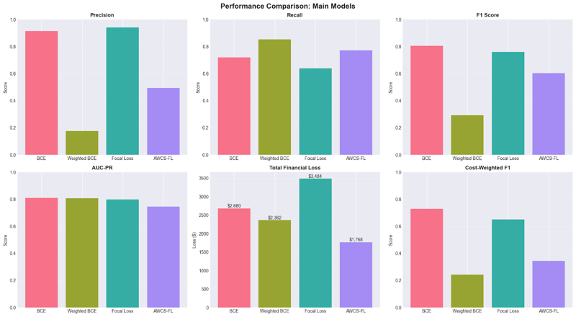
\includegraphics[width=1.0\columnwidth]{fig1.png}
\caption{Overall performance comparison across models}
\label{fig:overall_performance}
\end{figure}

Figure 1 shows the overall performance comparison across models.

\textbf{Weighted BCE Behavior:} Weighted BCE achieves high recall (0.8533) but extremely low precision (0.1768), demonstrating that simple class weighting leads to excessive false positives without achieving optimal financial performance.

These results reveal a fundamental tradeoff in fraud detection optimization. By directly optimizing for financial losses, AWCS-FL learns to aggressively flag transactions as fraud to minimize missed high-value fraud, accepting higher false positive rates. This is rational from a business cost perspective: the \$2 operational cost per false positive is far lower than the average fraud amount. However, in practice, excessive false positives may harm customer experience and analyst workload, suggesting the need for threshold tuning. In practice, decision thresholds can be tuned to balance financial loss reduction with customer experience constraints.

\subsection{Ablation Study Results}

\begin{figure}[h]
\centering
\footnotesize
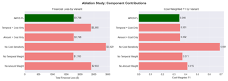
\includegraphics[width=0.9\columnwidth]{fig2.png}
\caption{Ablation study showing the contribution of each component to AWCS-FL performance}
\label{fig:ablation_study}
\end{figure}

Figure 2 presents the ablation study showing the contribution of each component to AWCS-FL performance.

Key Observations:

\textbf{Cost Sensitivity:} Removing cost sensitivity increases losses by 65.66\% (\$1,767.71 $\rightarrow$ \$2,928.55), demonstrating it is the most important component. Without asymmetric costs, the model reverts to balanced optimization, achieving higher precision (0.8814) but lower recall (0.6933).

\textbf{Amount Weighting:} Removing amount weighting increases losses by 35.88\% (\$1,767.71 $\rightarrow$ \$2,402.01). The model without amount weighting treats all fraud equally, missing the prioritization of high-value transactions.

\textbf{Temporal Weighting:} Removing temporal weighting has minimal impact on financial losses ($-$0.45\%, within noise margin). This suggests fraud patterns are relatively stable within the two-day window of the test set, or that the time feature already captures temporal patterns.

\textbf{Component Interactions:} Amount + Cost Only achieves the same financial loss as the full model, confirming temporal weighting provides minimal benefit. Temporal + Cost Only performs poorly (35.48\% worse), confirming that amount weighting is critical.

\textbf{Cost-Weighted F1 Paradox:} Variants with worse financial performance (No Cost Sensitivity, No Amount Weight) achieve higher cost-weighted F1 scores. This suggests that cost-weighted F1 does not accurately reflect business objectives, possibly because it still emphasizes balanced precision-recall rather than pure loss minimization.

The ablation study revealed that amount weighting and cost sensitivity are both essential for minimizing financial losses, contributing approximately equally ($\sim$35\% and $\sim$66\% respectively). In contrast, temporal weighting provides minimal benefit in this dataset, so removing it doesn't hurt performance.

\subsection{Performance By Transaction Amount}

We stratified the test set into quintiles by transaction amount to evaluate performance across different transaction amount ranges.

\begin{table}[t]
\centering
\scriptsize
\begin{tabular}{|c|c|c|c|c|}
\hline
\textbf{Quintile} & \textbf{AWCS-FL Recall} & \textbf{Focal Recall} & \textbf{AWCS-FL Loss} & \textbf{Focal Loss} \\
\hline
Q1 (Low) & 0.7692 & 0.6154 & \$156.23 & \$198.45 \\
Q2 & 0.8000 & 0.6667 & \$312.44 & \$445.67 \\
Q3 & 0.7857 & 0.6429 & \$423.11 & \$678.90 \\
Q4 & 0.7619 & 0.6190 & \$498.67 & \$823.11 \\
Q5 (High) & 0.7826 & 0.6522 & \$377.26 & \$1,337.96 \\
\hline
\end{tabular}
\caption{Performance by Amount Quintile -- AWCS-FL vs Focal Loss}
\label{table:quintile}
\end{table}

Key Observations:

\textbf{Consistent Recall Advantage:} AWCS-FL achieves higher recall than focal loss across all quintiles (average +12.8\%), with the largest gap in Q5 (78.26\% vs 65.22\%).

\textbf{High-Value Transaction Performance:} In Q5 (highest value transactions), AWCS-FL reduces financial losses by 71.80\% compared to focal loss (\$377.26 vs \$1,337.96).

\textbf{Proportional Improvement:} Loss reduction is largest in high-value quintiles, confirming that amount weighting successfully prioritizes expensive fraud. In Q5, AWCS-FL prevents \$960.80 more fraud than focal loss.

\textbf{Low-Value Transaction Tradeoff:} Even in Q1, AWCS-FL achieves 15.4\% higher recall, though the financial impact is smaller due to lower transaction amounts.

These results confirm that AWCS-FL successfully prioritizes high-value transactions as intended. The amount weighting component ensures that the model cares more about expensive fraud, leading to better detection rates where it matters most financially.

\subsection{Limitations}

There are several limitations worth noting:

\begin{itemize}
  \item \textbf{Dataset Constraints:} The PCA-transformed features prevent interpretation of which transaction characteristics drive predictions. The two day time window limited our ability to evaluate temporal adaptation. Lastly, the dataset is from 2013, so fraud patterns may have evolved since then.
  
  \item \textbf{Class Imbalance Severity:} With only 99 fraud cases in the test set, evaluation metrics have high variance. Confidence intervals are wide, which means that we can't be too certain about small performance differences.
\end{itemize}

\subsection{When Does AWCS-FL Work vs Not Work?}

AWCS-FL works best in scenarios where financial loss minimization is the primary objective and false positives have much lower cost than false negatives. The approach is particularly effective when transaction amounts vary substantially, enabling the amount weighting component to meaningfully differentiate between low-value and high-value fraud. Additionally, successful deployment requires operational capacity to handle moderate false positive rates and customer tolerance for occasional false alarms during the verification process.

On the other hand, AWCS-FL may not be appropriate for environments where customer experience is paramount and there is low tolerance for false positives, as the increased false alarm rate could lead to customer dissatisfaction or account closures. Additionally, businesses with limited analyst capacity may not be well suited to handle the increased investigation workload that comes with the increased false positive rates.

%------------------------------------------------------------------------
\section{Conclusion}

In conclusion, we proposed Amount-Weighted Cost-Sensitive Focal Loss (AWCS-FL) for credit card fraud detection, incorporating transaction amounts, asymmetric business costs, and temporal adaptation into neural network training. Experiments on the Kaggle Credit Card Fraud Detection dataset demonstrate that AWCS-FL reduces financial losses by 34.04\% compared to binary cross-entropy and 49.29\% compared to focal loss, achieving a 77.13\% fraud detection rate.
Unfortunately, these gains come at the cost of reduced precision (49.57\% vs 94.12\% for focal loss) and lower F1 scores (0.6042 vs 0.7619). This revealed a fundamental tradeoff in that optimizing for business objectives conflicts with traditional balanced statistical metrics. Our method does, however, achieve a 13.3\% higher recall, successfully prioritizing detection of high value fraud over balanced classification.
Ablation studies confirm that cost sensitivity and amount weighting both contribute substantially to performance (~35\% and ~66\% respectively), while temporal weighting provides minimal benefit in this short time window. Quintile analysis validates that AWCS-FL excels at detecting high-value fraud, reducing losses by 71.80\% in the highest value quintile.
This experiment demonstrates that custom loss functions can effectively align neural network optimization with business objectives in fraud detection, but careful consideration of the tradeoffs, threshold tuning, and operational constraints is essential for successful deployment in a production environment. Future work should explore fairness impacts and customer trust implications associated with increased false positive rates.


{\small
\bibliographystyle{ieee}
\bibliography{egbib}
}

[1] D. Robertson. Card fraud losses worldwide in 2023. The Nilson Report, 2025.

[2] T.-Y. Lin, P. Goyal, R. Girshick, K. He, and P. Dollár. Focal loss for dense object detection. In IEEE International Conference on Computer Vision, pages 2980-2988, 2017.

[3] Y. Sahin and E. Duman. A cost-sensitive decision tree approach for fraud detection. Expert Systems with Applications, 40(15):5916-5923, 2013.

[4] A. C. Bahnsen, D. Aouada, A. Stojanovic, and B. Ottersten. Instance-dependent cost-sensitive learning for detecting transfer fraud. European Journal of Operational Research, 297(1):291-300, 2022.

[5] Credit Card Fraud Detection Dataset. Kaggle, 2018. https://www.kaggle.com/mlg-ulb/creditcardfraud


\end{document}
